\documentclass[a4paper,twocolumn,landscape]{article}
\usepackage{geometry}
\usepackage{concmath}
\usepackage[OT1]{fontenc}
\usepackage{graphicx}
\usepackage{amsfonts}
\usepackage{amsmath}
\usepackage{calrsfs}
\usepackage{color}
\usepackage[dvipsnames]{xcolor}
\usepackage[many]{tcolorbox}
\usepackage{setspace}              
\usepackage{multicol}  
\geometry{margin=0.4in}
\usepackage{listings}

\usepackage{xcolor}

\definecolor{codegreen}{rgb}{0,0.6,0}
\definecolor{codegray}{rgb}{0.5,0.5,0.5}
\definecolor{codepurple}{rgb}{0.58,0,0.82}
\definecolor{backcolour}{rgb}{0.95,0.95,0.92}

\lstdefinestyle{mystyle}{
    basicstyle=\ttfamily\footnotesize,
    breakatwhitespace=false,         
    breaklines=true,                 
    captionpos=b,                    
    keepspaces=true,                 
    numbers=left,                    
    numbersep=5pt,                  
    showspaces=false,                
    showstringspaces=false,
    showtabs=false,                  
    tabsize=2
}

\lstset{style=mystyle}


\begin{document}

\begin{lstlisting}[language=Python]
import numpy as np
from scipy import signal
import matplotlib.pyplot as plt

#avec 200 points le signal est visiblement legerement trapezoide
t_e = np.linspace(0, 0.02, 2000, endpoint=False) 
t = np.linspace(0, 0.02, 200, endpoint=False)

T = 3e-3
f = 1/T
omega_c = 200
T_e = 0.02/200
H_0 = 0.5

e = signal.square(2 * np.pi * f * t_e, duty=2/3)
e = ((e+1)*4.5)/2

#e a 10x plus de points
def recurrence(s, n, res):
    return (1-omega_c*T_e)*s[n] + H_0 * T_e * omega_c * e[n*res]

def u_s(l):
    s = np.zeros(l)
    s[0] = 1
    n = 2000//l
    for i in range(0, l-1):
        s[i+1] = (1-omega_c*T_e)*s[i] + H_0 * T_e * omega_c * e[i*n]
    return s

s_1 = u_s(200)
s_2 = u_s(2000)


plt.plot(t_e, e)
plt.plot(t, s_1)
plt.plot(t_e, s_2)

plt.title("Filtrage passe-bas du signal creneau")
plt.xlabel("t (s)")
plt.ylabel("Amplitude (V)")

plt.ylim(-0.2, 5)

plt.legend(['signal entree', 'signal filtre N = 200', 'signal filtre N = 2000'], loc="upper left") 

plt.grid()
plt.show()    
\end{lstlisting}

\newpage
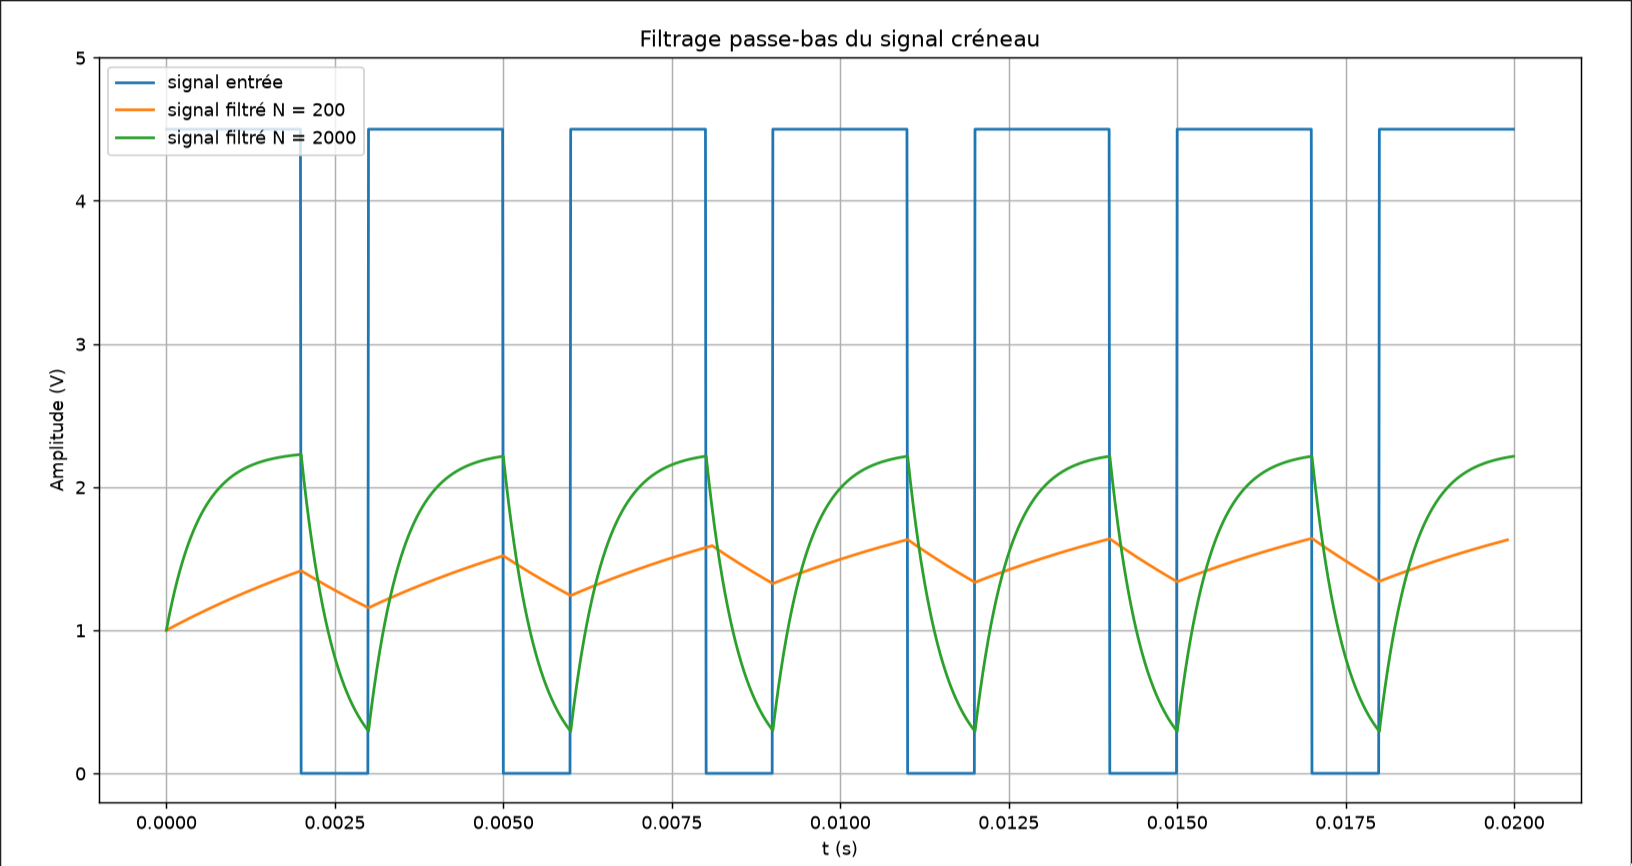
\includegraphics[scale=0.25]{graphe.png}

\end{document}